\section{Method: Similarity-Calibrated Conformal prediction}\label{sec:method}
SCC is a drop-in modification of split conformal prediction that makes the calibration transferable
across operating regimes. It runs in two stages (Fig.~\ref{fig:overview}): offline, on a source asset
with run-to-failure data, it calibrates a conformal quantile in a dimensionless coordinate; online, on
a target asset in a different regime and with no failure history, it re-scales that quantile by the
target's physical scale to produce a certified RUL lower bound. The only quantities crossing from
source to target are the scale-free conformal quantile and the target's physical scale, so no target
failure data is needed.

\begin{figure}[t]\centering
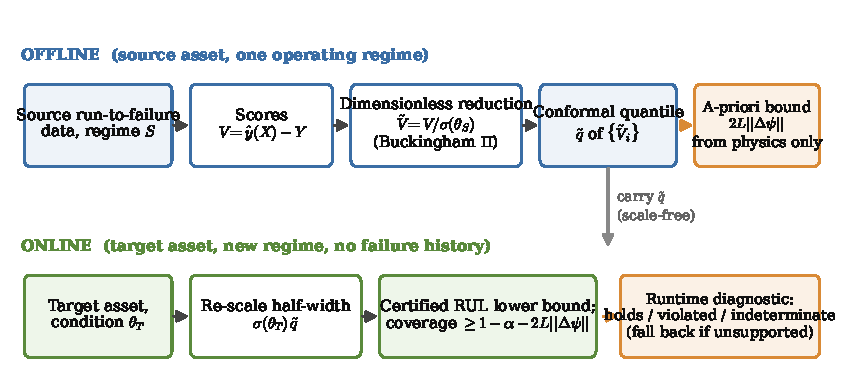
\includegraphics[width=\linewidth]{figures/fig_overview.pdf}
\caption{The SCC workflow. Offline, source scores are made dimensionless by a physics-derived scale
$\sigma(\theta_S)$ and a conformal quantile $\tilde q$ is taken. Online, the quantile is
re-dimensionalised by the target scale $\sigma(\theta_T)$ to give a certified RUL lower bound. The
coverage shortfall is bounded a priori from physical parameters, and a runtime diagnostic reports
whether the similitude premise is supported.}\label{fig:overview}
\end{figure}

\subsection{Setup and the SCC procedure}\label{sec:procedure}
Units are indexed by operating condition $c$ with known physical parameters $\theta_c$ (load, speed,
temperature). A unit yields features $X$ and true RUL $Y$ with joint law $\mathbb P_c$; a pre-trained
predictor $\hat y$ and the one-sided over-prediction score $V=\hat y(X)-Y$ (a lower RUL bound) have
score law $\law c$. The procedure is:
\begin{enumerate}
\item \emph{Dimensionless calibration.} On calibration data $\{(X_i,Y_i)\}_{i=1}^n$ drawn from the
source regime $S$, form scores $V_i=s(X_i,Y_i)$ and divide by the source scale to obtain dimensionless
scores $\tilde V_i=V_i/\sigma(\theta_S)$.
\item \emph{Conformal quantile.} Take $\tilde q=\tilde V_{(\lceil(1-\alpha)(n+1)\rceil)}$, the order
statistic giving the empirical $(1-\alpha)$ quantile of the dimensionless scores.
\item \emph{Re-dimensionalised deployment.} For a target unit under condition $T$, return the RUL set
$\mathcal C(X_{n+1})=\{y:s(X_{n+1},y)\le\sigma(\theta_T)\,\tilde q\}$, re-scaling the quantile by the
\emph{target} scale.
\end{enumerate}
Naive (regime-blind) conformal is the special case $\sigma\equiv1$; it applies the source quantile
directly to the target and miscovers whenever $\sigma(\theta_S)\neq\sigma(\theta_T)$. The single
change in SCC is calibrating and deploying in the $\sigma$-normalised coordinate.

\subsection{The dimensionless scale and what it absorbs}\label{sec:scale}
The scale $\sigma(\theta_c)$ comes from the governing physics through the Buckingham $\Pi$ theorem,
which yields dimensionless groups. These split into scale-setting groups, used to form a
characteristic score scale $\sigma(\theta_c)>0$ such that the dimensionless score
$\tilde V=V/\sigma(\theta_c)$ has a condition-invariant law under exact similitude, and a residual
\emph{similitude-departure} parameter $\boldsymbol\psi(\theta_c)\in\mathbb R^m$ collecting the groups
the scale does not absorb (unmodelled physics). When the dimensionless model is complete,
$\boldsymbol\psi$ is constant across conditions.

Two standard degradation laws show what the scale removes. For rolling-contact fatigue
(Lundberg--Palmgren / ISO~281~\cite{lundberg1947dynamic,iso281}, rating life $\propto(C/P)^p$ with
$p=3$), the scale $\sigma=T_L\propto(C/P)^p/n$ \emph{absorbs} the load--speed group $P/C$. For
first-order catalyst deactivation (Arrhenius $k=A\,e^{-E/RT}$~\cite{levenspiel1999chemical,perry2008handbook}),
the scale $\sigma=1/k_{\mathrm{nom}}$ \emph{contains} the primary rate group $e^{-E/RT}$. In both
cases a large difference in the dominant operating parameter is taken up by $\sigma$ and does not by
itself induce a mismatch in the score distribution; what remains is only the residual departure
$\boldsymbol\psi$.

\subsection{Coverage guarantee}\label{sec:guarantee}
Calibrating in the dimensionless coordinate restores coverage up to a term set by the physical
departure. With calibration drawn i.i.d.\ from the source $S$ and a target point
$(X_{n+1},Y_{n+1})\sim\mathbb P_T$ independent of calibration, the SCC interval of
Section~\ref{sec:procedure} satisfies
\begin{equation}\label{eq:cert}
\mathbb P\big(Y_{n+1}\in\mathcal C(X_{n+1})\big)\;\ge\;
1-\alpha-2L\lVert\boldsymbol\psi(\theta_S)-\boldsymbol\psi(\theta_T)\rVert,
\end{equation}
where $\lVert\Delta\boldsymbol\psi\rVert=\lVert\boldsymbol\psi(\theta_S)-\boldsymbol\psi(\theta_T)\rVert$
is the similitude departure between the regimes and $L$ is a Lipschitz constant estimated from source
data (Section~\ref{sec:estL}). Equation~\eqref{eq:cert} follows by composing the dimensionless
reduction with the non-exchangeable conformal bound of Barber et al.~\cite{barber2023conformal}; the
formal statement, hypotheses, and proof are collected in~\ref{app:proof}. Here we read off its
engineering content.

The departure $\lVert\Delta\boldsymbol\psi\rVert$ is a physical quantity, not a function of target
failure data, which gives two regimes of use. Under complete similitude ($\boldsymbol\psi$ constant)
the bound is zero and coverage is at least $1-\alpha$ for \emph{arbitrarily large} differences in the
scale-setting parameters, needing only the target scale $\sigma(\theta_T)$; this is the property a
newly commissioned asset can rely on. Under incomplete similitude, coverage is certified down to
$1-\alpha-2L\lVert\Delta\boldsymbol\psi\rVert$ once the departure is bounded, so the worst-case
shortfall is known before deployment. Neither case estimates a density ratio, which is what separates
SCC from weighted and covariate-shift conformal.

\subsection{Estimating the departure sensitivity $L$}\label{sec:estL}
The constant $L$ in~\eqref{eq:cert} is obtained from source data alone. With $m\ge2$ source
conditions, regress the empirical total-variation distance between dimensionless score laws,
$\dtv(\tilde{\mathcal V}_S,\tilde{\mathcal V}_{S'})$, on the physical departure
$\lVert\Delta\boldsymbol\psi\rVert$ over source pairs; the slope estimates $L$ and the intercept $a$
estimates the finite-sample floor, which decays as $n^{-1/2}$. The operational bound
$2(a+L\lVert\Delta\boldsymbol\psi\rVert)$ then upper-bounds the target coverage gap using only
source-side information.

\subsection{Runtime similitude diagnostic}\label{sec:diagnostic}
The guarantee~\eqref{eq:cert} is conditional on the similitude premise, which bites only when
$\boldsymbol\psi$ varies across conditions. Because exact similitude makes the dimensionless life
condition-invariant, the premise is testable from source data, and SCC carries a runtime check that
acts as a go/no-go monitor. For each condition pair it forms
$g=\mathrm{median}(D\mid c)/\mathrm{median}(D\mid c')$, where $D$ is the dimensionless life (the
dynamic-capacity constant cancels), equivalently the empirical median-life ratio divided by the L10
prediction. A bootstrap confidence interval on $g$ yields a three-way verdict: $1$ inside a tight
interval gives \emph{holds}; $1$ outside gives \emph{violated}; an interval wider than a preset fold
gives \emph{indeterminate} (underpowered). On the latter two, SCC declines the a-priori certificate
and falls back to data-driven conformal, so an unsupported premise produces a conservative fallback
rather than a silent miscoverage.
